\part{Arrays and lists}
\frame{\partpage}

\begin{frame}{Memory allocation --- recap}
	\begin{itemize}
		\pause\item Memory is allocated in \textbf{blocks}
		\pause\item The program specifies the size, in bytes, of the block it wants
		\pause\item The OS allocates a \textbf{contiguous} block of that size
		\pause\item The program owns that block until it frees it
		\pause\item Blocks can be allocated and deallocated at will, but can \textbf{never grow or shrink}
	\end{itemize}
\end{frame}

\begin{frame}{Collection types}
	\begin{itemize}
		\pause\item Memory management is hard and programmers are lazy
		\pause\item Collections are an \textbf{abstraction}
			\begin{itemize}
				\pause\item Hide the details of memory allocation, and allow the programmer to write simpler code
			\end{itemize}
		\pause\item Collections are an \textbf{encapsulation}
			\begin{itemize}
				\pause\item Bundle together the data's representation in memory along with the algorithms for accessing it
			\end{itemize}
	\end{itemize}
\end{frame}

\begin{frame}{Arrays}
	\begin{itemize}
		\pause\item An \textbf{array} is a contiguous block of memory in which objects are stored,
			equally spaced, one after the other
		\pause\item Each array element has an \textbf{index}, starting from zero
		\pause\item Given the address of the $0$th element, it is easy to find the $i$th element:
	\end{itemize}
	$$ \text{address}_i = \text{address}_0 + (i \times \text{elementSize}) $$
	\begin{itemize}
		\pause\item E.g.\ if the array starts at address $1000$ and each element is $4$ bytes,
			the 3rd element is at address $1000 + 4 \times 3 = 1012$
		\pause\item Accessing an array element is \textbf{constant time} $O(1)$
	\end{itemize}
\end{frame}

\begin{frame}{Lists}
	\begin{itemize}
		\pause\item An array is a block of memory, so its size is \textbf{fixed} once created
		\pause\item A \textbf{list} is a variable size array
		\pause\item When the list needs to change size, it \textbf{creates} a new array,
			\textbf{copies} the contents of the old array, and \textbf{deletes} the old array
	\end{itemize}
\end{frame}

\begin{frame}[fragile]{Arrays and lists in C\#}
	\begin{lstlisting}
int[] myArray = new int[10];

int[] myOtherArray = new int[] { 2, 3, 5, 7, 11 };

List<int> myList = new List<int>();

List<int> myOtherList = new List<int> { 2, 3, 5, 8, 13 };
	\end{lstlisting}
\end{frame}

\begin{frame}{Time taken to append an element to a list of size $n$}
	\begin{center}
		\vspace{-5ex}
		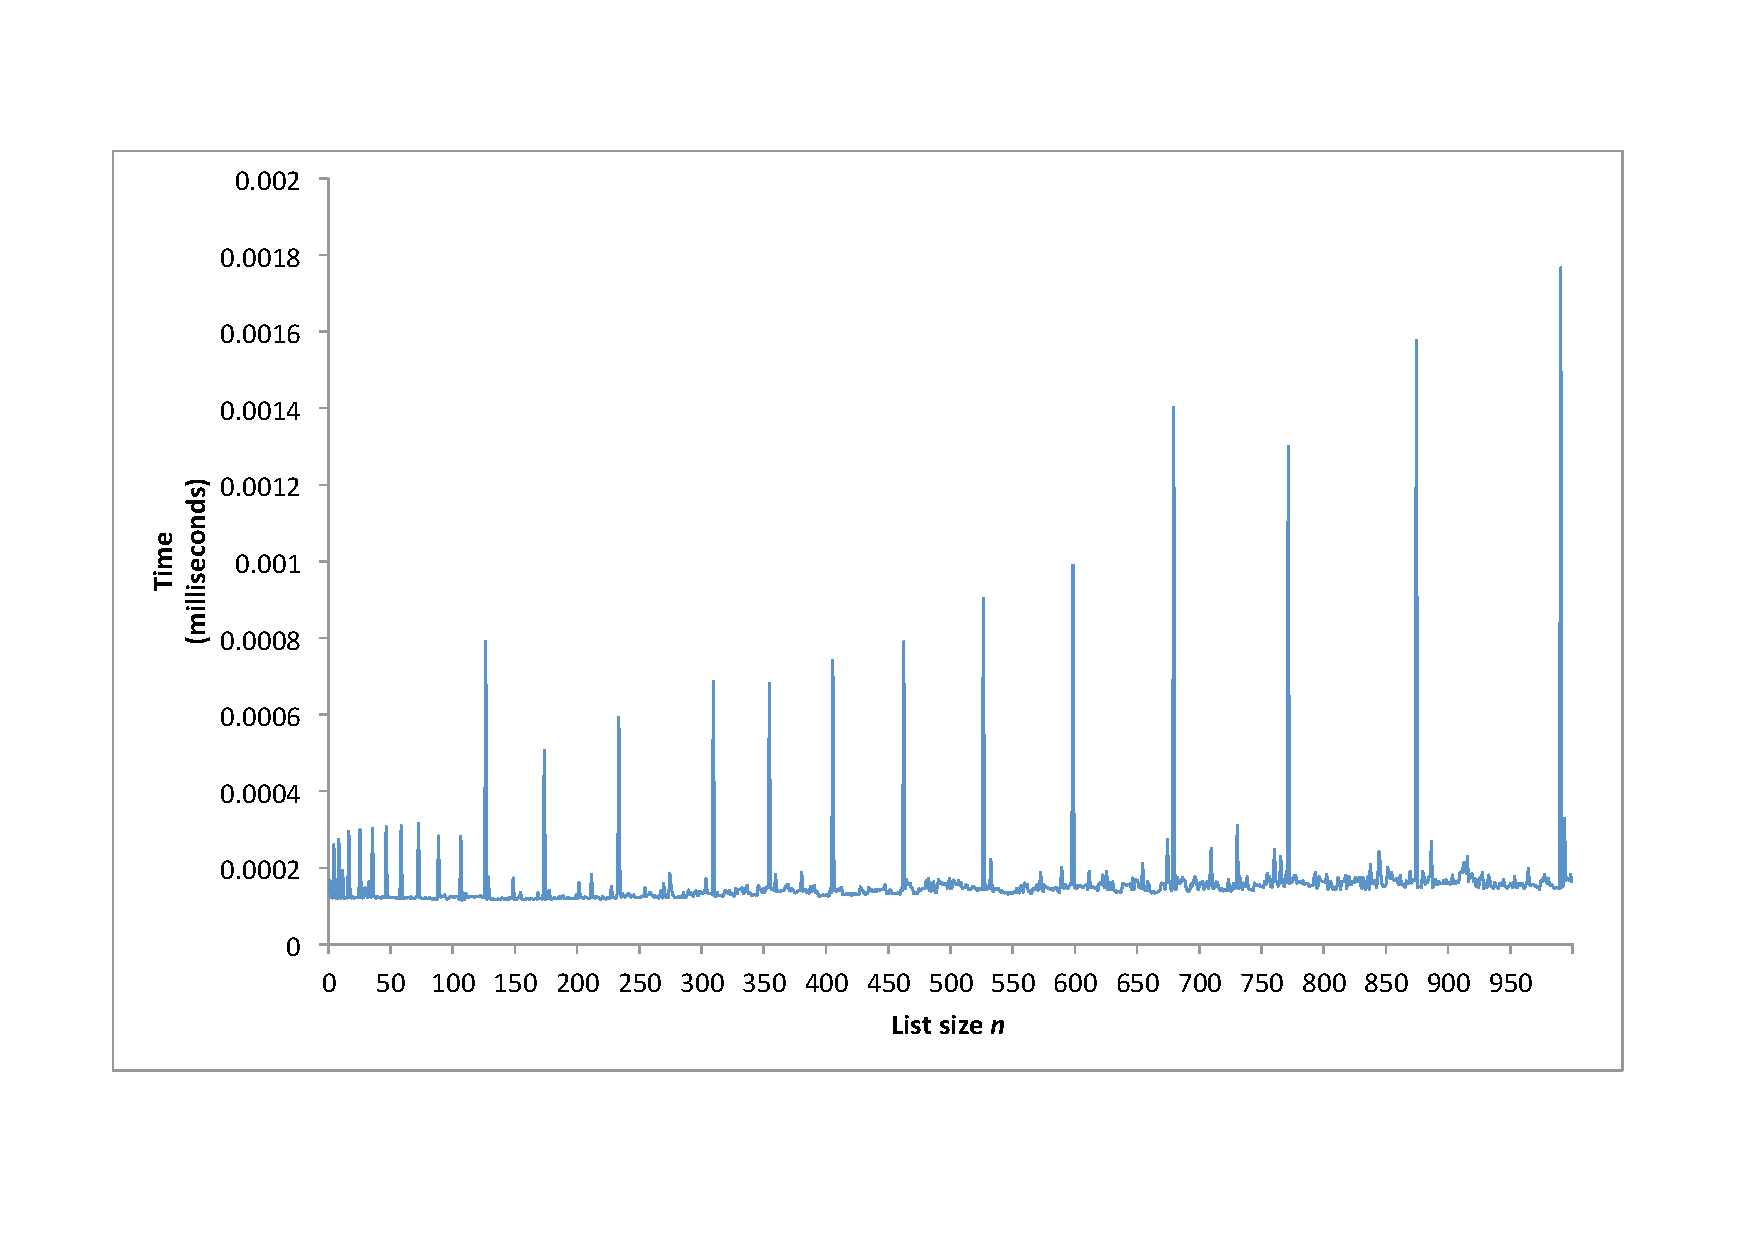
\includegraphics[height=0.9\textheight]{list_append_timing}
	\end{center}
\end{frame}

\begin{frame}{Operations on lists}
	\begin{itemize}
		\pause\item \textbf{Appending} to a list is \textbf{amortised constant time}
			\begin{itemize}
				\pause\item Usually $O(1)$, but can go up to $O(n)$ if the list needs to change size
			\end{itemize}
		\pause\item \textbf{Inserting} anywhere other than the end is \textbf{linear time}
			\begin{itemize}
				\pause\item Can't just insert new bytes into a memory block ---
					need to move all subsequent list elements to make room
			\end{itemize}
		\pause\item Similarly, \textbf{deleting} anything other than the last element is \textbf{linear time}
	\end{itemize}
\end{frame}
